\documentclass[main.tex]{subfiles}
\begin{document}

\chapter{Hardware Setup}
	\section{Overview}
	[DONT FORGET TO SPELL CHECK]
	Constructing a thermistor[?] circuit is a simple process requiring  very few parts. The parts
	used in this report are:
	[INSERT LIST OF PARTS, be specific]
	Blah Blah Blah...
	
	
	\section{Programmer}
	To program a microcontroller, a programmer will be needed. The programmer used in this report
	will be the Dragon. Setting up the Dragon requires a USB connection to the computer where
	the program will be uploaded from and wiring the programmer pins to microcontroller pins
	as shown in [MISSING FIGURE].
	\begin{figure}[H]
		\begin{center}
			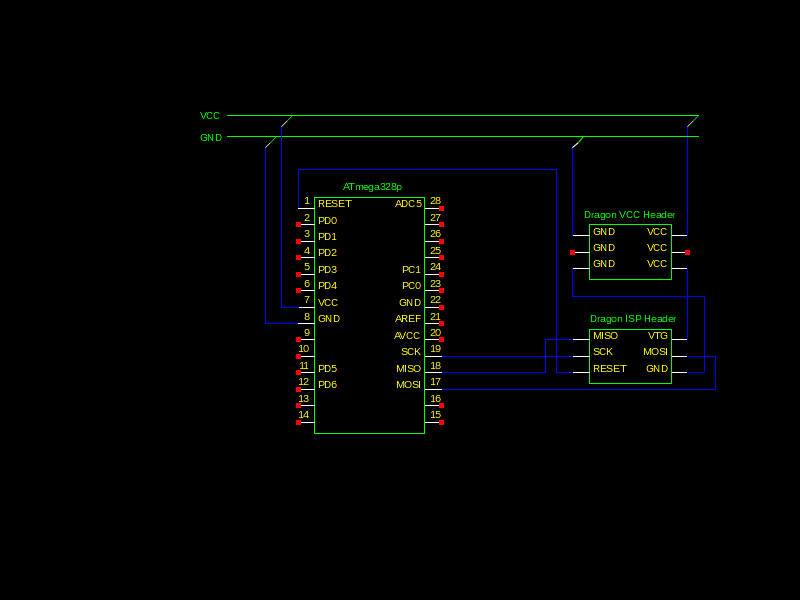
\includegraphics[width=\linewidth]{programmer}
		\end{center}
		\caption{}
		\label{fig:test}
	\end{figure}	


	\section{Seven-Segment Display}
		\subsection{General I/O}
		When a pin on the ATmega328p is set high, it will supply 5 volts on that pin. To power an
		LED as common anode, the forward voltage drop and the operating current must be known.
		The value of the resistor in series with the LED then becomes: \[(5 - V_f)/I_f\]
		
		The seven-segment display consistes of seven of these circuits per digit. That will be two sets
		of seven in common anode. In common anode, all seven segments share a common 5V and setting the
		pin that matches the segment low will turn the LED on sinking current into the ATmega.
		
		
		\subsection{Mapping}
		Having the display show a number requires powering the segments that correspond to that digit.
		The pin layout for the seven-segment display used in this report is shown in [MISSING FIGURE].
		So to display the number 4 on the left digit, pin 4 must be high for common anode and pins
		14, 13, 16, and 1 must be low while the rest are high.
		\begin{figure}[H]
			\begin{center}
				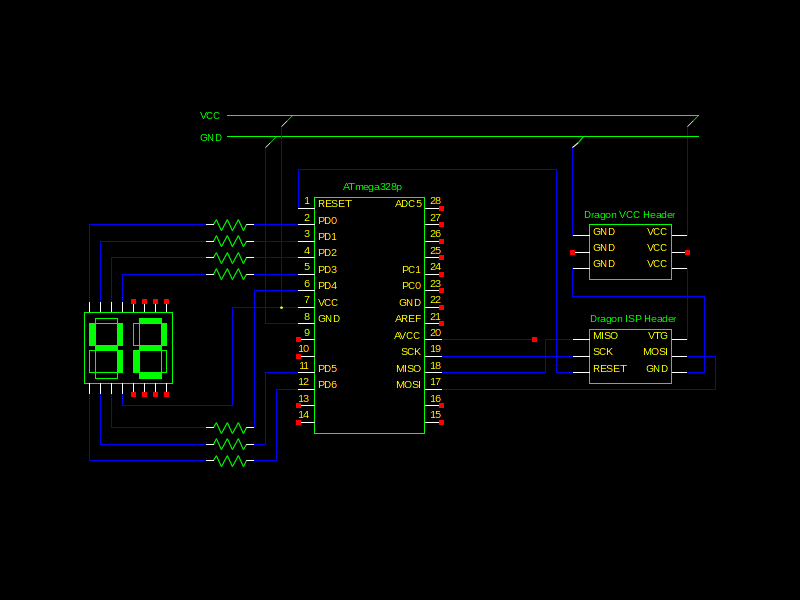
\includegraphics[width=\linewidth]{mapping}
			\end{center}
			\caption{7seg DATASHEET}
			\label{fig:whatIsThis}
		\end{figure}
		
		\subsection{Digit Pulsing}
		Controlling 14 LEDs with the ATmega would require 14 pins if every pin would control a single
		segment for both digits, but by alternating which digit is powered after every few clock cycles,
		the number of pins can be reduced to 9 (7 for the segments, and 2 for turning the digits on/off
		via the common anode pins). The new circuit is shown in [MISSING FIGURE].
		\begin{figure}[H]
			\begin{center}
				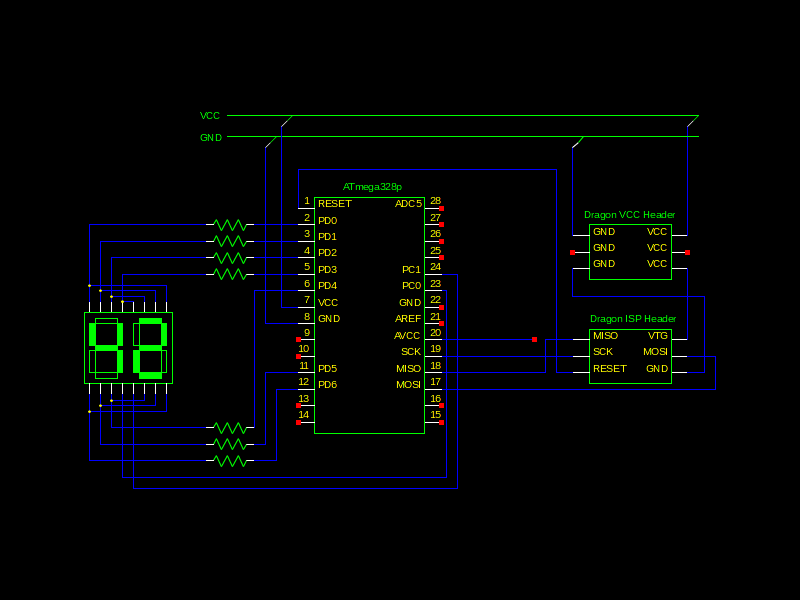
\includegraphics[width=\linewidth]{pulsing}
			\end{center}
			\caption{Both Digits Wired in Parallel}
			\label{fig:whatIsThis}
		\end{figure}
		
	\section{ADC}
	The ADC module of the ATmega is powered by three seperate pins (20, 21, 22). The circuit for
	these pins is shown in [BLAH BALH FIGURE]. [NEED TO FINISH]
	\begin{figure}[H]
		\begin{center}
			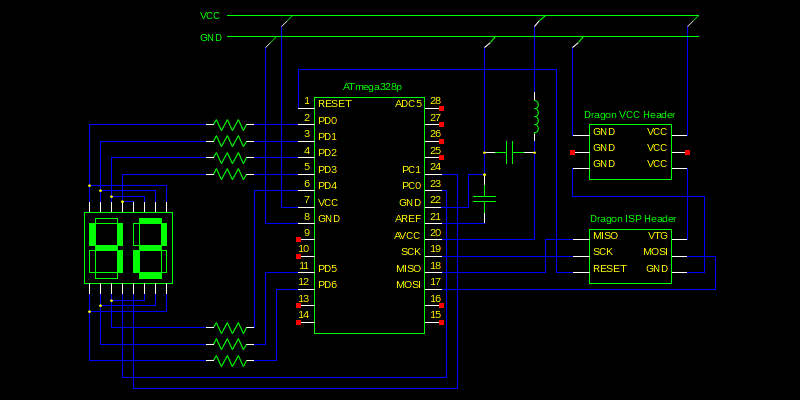
\includegraphics[width=\linewidth]{adcPower}
		\end{center}
		\caption{ADC Power Added}
		\label{fig:whatIsThis}
	\end{figure}

	\section{Thermistor}
	The ADC module reads from a pin determined in the program. In this report ADC5 (pin 28) is used
	with the thermistor setup shown in [MISSING FIGURE]. The ADC measures the varying voltage drop
	across the thermistor and the program will then match that to its corresponding temperature.
	\begin{figure}[H]
		\begin{center}
			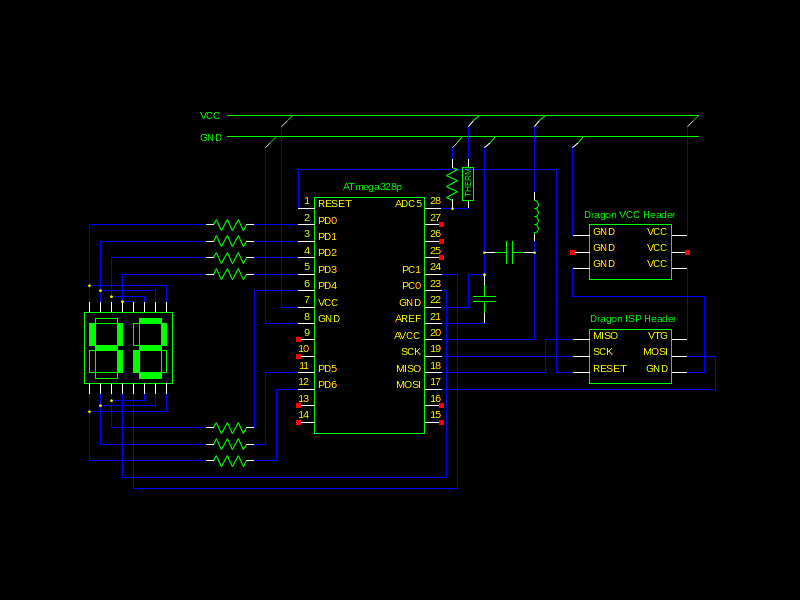
\includegraphics[width=\linewidth]{Thermistor}
		\end{center}
		\caption{Completed Thermistor Circuit}
		\label{fig:ascSA}
	\end{figure}
\end{document}
